\documentclass[11pt]{article}
\usepackage[margin=1in]{geometry}
\usepackage{booktabs}
\usepackage{amsmath}
\usepackage{amssymb}
\usepackage{graphicx}
\usepackage[colorlinks=true,linkcolor=blue,citecolor=blue]{hyperref}

\renewcommand{\thetable}{S\arabic{table}}
\renewcommand{\thefigure}{S\arabic{figure}}
\renewcommand{\thesection}{S\arabic{section}}

\title{Supplementary Material\\
\large Deep Neural Network Surrogates for Approximate Bayesian Computation:\\
A Simulation Study for Mutation-Rate Estimation\\
in Markov Branching Processes}
\author{}
\date{}

\begin{document}
\maketitle

\noindent \textbf{Journal:} Statistics and Computing (submitted).
\textbf{Corresponding author:} Sachin Letchumanan, Department of Statistics, Virginia Tech, Blacksburg, VA 24061, USA (sachin.letchumanan@gmail.com).

\noindent This document contains the full architecture-, activation- and capacity-search tables for Study I
(Section S1) and, for Study II, the full architecture search (S2), the GPS-ABC runs (S3), the check of our
data generator against the training sets released by the original authors (S4) and the calibration rank
histograms (S5). Each table below corresponds to a numbered claim in the main text; the surrounding prose
there states the headline conclusion and is not repeated here except as needed to make each table self-contained.

\section{Study I: the full activation, normalisation and capacity search}
\label{ssec:s1-1d-arch}

The deployed one-dimensional surrogate (Section~4.1 of the main text) is a
shallow funnel multilayer perceptron, input $\theta=\log_{10}p$, two
GELU-activated dense layers at width $32$--$16$ ($626$ parameters). That
choice is the outcome of the two-stage search reported in full here:
activation/normalisation first, at a $128$--$64$ baseline, then capacity,
once the activation question was settled.

\begin{table}[h]
\centering
\caption{Architecture search, one-dimensional model: mean-curve fit MSE
against the denoised response curve (irreducible replicate-noise floor
$\approx 4.7\times 10^{-3}$).}
\label{stab:arch1D}
\resizebox{\linewidth}{!}{%
\begin{tabular}{lrr}
\toprule
Model & Mean-curve MSE & vs.\ GP \\
\midrule
Gaussian process (GPS-ABC baseline) & $3.836\times10^{-4}$ & --- \\
\textbf{DNN, GELU (128, 64), no BatchNorm [selects activation]} & $\mathbf{3.888\times10^{-4}}$ & $+1\%$ \\
DNN ensemble $\times 5$, SiLU (128, 128, 64) & $3.960\times10^{-4}$ & $+3\%$ \\
DNN ensemble $\times 5$, tanh (256, 128) & $4.178\times10^{-4}$ & $+9\%$ \\
DNN, SiLU (128, 128, 64) & $4.400\times10^{-4}$ & $+15\%$ \\
DNN, tanh (64, 64, 32) & $4.435\times10^{-4}$ & $+16\%$ \\
DNN, tanh (256, 128) & $4.503\times10^{-4}$ & $+17\%$ \\
DNN, ReLU + BatchNorm + dropout (64, 64, 32) & $4.352\times10^{-3}$ & $+1035\%$ \\
\bottomrule
\end{tabular}%
}
\end{table}

The row that determines every downstream comparison in the main text is the
last one: an otherwise-reasonable network carrying BatchNorm and dropout fits
\emph{eleven times worse} than the same network without them. BatchNorm
normalises per-minibatch statistics, useful in deep classification networks;
but on a smooth scalar regression over a one-sided domain (the $\theta$-grid
has a hard edge at $-8$) it injects batch-dependent noise and biases
predictions near that boundary. A follow-up ablation isolating only the
activation function (same 128--64 architecture, no BatchNorm, averaged over
three random seeds) found ReLU, SiLU, GELU, and tanh within $7\%$ of one
another ($3.95$--$4.23\times10^{-4}$): a statistical tie, with ReLU
marginally ahead. Because accuracy does not separate them, the choice of
GELU is made on structural grounds (smoothness, immunity to the dead-neuron
failure mode) at no measurable accuracy cost. A second search round using
$7$-network deep ensembles (mean-curve MSE $3.94$--$4.25\times10^{-4}$
across four ensemble configurations) did not improve on the single chosen
network, so the simpler model is retained throughout.

\begin{table}[h]
\centering
\caption{One-dimensional model: does capacity matter? Curve MSE is
against the denoised response curve, mean over three seeds. Downstream
MSE and 95\% CI length are DNN-ABC at the same scale as the main text's
mean-squared-error table ($40$ replicates/cell, full $p\times J$ grid), one
seed per row.}
\label{stab:capacity1D}
\setlength{\tabcolsep}{4.5pt}
\resizebox{\linewidth}{!}{%
\begin{tabular}{lrrrr}
\toprule
Hidden layers & Parameters & Curve MSE ($\times$ GP) & Downstream MSE & Downstream 95\% CI \\
\midrule
GP (GPS-ABC baseline) & --- & $3.836\times10^{-4}$ (---) & $2.702\times10^{-6}$ & $2.137\times10^{-3}$ \\
\textbf{32--16 (deployed)} & \textbf{626} & $\mathbf{3.896\times10^{-4}}$ ($\mathbf{+1.6\%}$) & $\mathbf{1.433\times10^{-6}}$ & $\mathbf{1.300\times10^{-3}}$ \\
128--64 (original) & $8{,}642$ & $4.129\times10^{-4}$ ($+7.6\%$) & $1.514\times10^{-6}$ & $1.308\times10^{-3}$ \\
64--32 & $2{,}274$ & $3.957\times10^{-4}$ ($+3.2\%$) & $1.565\times10^{-6}$ & $1.377\times10^{-3}$ \\
16 (1 layer) & $66$ & $4.460\times10^{-4}$ ($+16.3\%$) & $1.579\times10^{-6}$ & $1.375\times10^{-3}$ \\
8 (1 layer) & $34$ & $4.983\times10^{-4}$ ($+29.9\%$) & $1.668\times10^{-6}$ & $1.393\times10^{-3}$ \\
16--8 & $186$ & $4.508\times10^{-4}$ ($+17.5\%$) & $1.810\times10^{-6}$ & $1.528\times10^{-3}$ \\
Linear (control) & $4$ & $4.672\times10^{-4}$ ($+21.8\%$) & --- & --- \\
\bottomrule
\end{tabular}%
}
\end{table}

On raw curve fit, capacity is not merely unnecessary above a small
threshold: it is mildly \emph{counter-productive} at the original size:
$128$--$64$ has the largest gap to the GP of any two-layer candidate tested
($+7.6\%$), while $32$--$16$, at $14\times$ fewer parameters, comes closest to
matching it ($+1.6\%$). On the downstream task the surrogate is actually
used for, $32$--$16$ is also the best point estimate on both accuracy and
interval length of every candidate tested, $128$--$64$ included, though
attaching Monte Carlo standard errors to the gap shows this specific edge is
not itself resolved (all nine $\Delta/\mathrm{SE}$ values fall below $0.6$ in
magnitude). Nothing in the data argues against the smaller network either:
$32$--$16$ never does measurably worse than $128$--$64$ in any cell. Only the
linear control shows a clear, unambiguous cost, confirming some nonlinearity
is required, just not much capacity beyond that.

\section{Study II: the full architecture search}
\label{ssec:s2-arch}

Twelve architectures, five seeds each, on the four-parameter data ($10{,}000$ design points $\times$ $5$ replicates; split by design
point $80/10/10$). Validation loss is the sum of the cross-entropy of the zero head and the Gaussian negative log-likelihood of
the two features (standardised); the test columns are on held-out design points and were never used for selection. RMSE is in
$\log_{10}$ units. Selection: best mean validation loss, then the cheapest model within one standard error of it.

\begin{table}[h]
\centering
\caption{Study II: full architecture search (mean over five seeds; $\pm$ s.d.\ for the validation loss).}
\label{stab:arch4D}
\scriptsize
\begin{tabular}{lrrrrrrrr}
\toprule
Surrogate & Params & Val.\ loss & Test NLL & RMSE $\log_{10}\bar d$ & RMSE $\log_{10}s$ & Zero log-loss & Train s & Epochs \\
\midrule
ResNet 3$\times$128 (GELU) & 100{,}357 & -3.3416$\,\pm\,$0.0038 & -2.901 & 0.1025 & 0.1076 & 0.0533 & 588 & 117 \\
MLP 4$\times$64 (GELU) & 13{,}125 & -3.3371$\,\pm\,$0.0048 & -2.907 & 0.1014 & 0.1074 & 0.0534 & 282 & 167 \\
MLP 3$\times$128 (SiLU) & 34{,}309 & -3.3280$\,\pm\,$0.0032 & -2.896 & 0.1015 & 0.1074 & 0.0539 & 343 & 160 \\
MLP 256--128--64 (GELU) & 42{,}757 & -3.3211$\,\pm\,$0.0041 & -2.887 & 0.1021 & 0.1074 & 0.0536 & 213 & 115 \\
ResNet 4$\times$256 (GELU) & 528{,}901 & -3.2958$\,\pm\,$0.0148 & -2.856 & 0.1035 & 0.1079 & 0.0541 & 2342 & 96 \\
MLP 128--64 (tanh) & 9{,}221 & -3.2924$\,\pm\,$0.0104 & -2.846 & 0.1047 & 0.1098 & 0.0553 & 296 & 207 \\
MLP 128--64 (GELU) & 9{,}221 & -3.2895$\,\pm\,$0.0131 & -2.853 & 0.1073 & 0.1090 & 0.0545 & 285 & 193 \\
MLP 64--32 (GELU/tanh) & 2{,}565 & -3.2841$\,\pm\,$0.0112 & -2.836 & 0.1049 & 0.1098 & 0.0554 & 261 & 251 \\
MLP 128--64 (SiLU) & 9{,}221 & -3.2750$\,\pm\,$0.0109 & -2.836 & 0.1104 & 0.1106 & 0.0547 & 331 & 198 \\
MLP 128--64 (ReLU) & 9{,}221 & -3.2702$\,\pm\,$0.0156 & -2.831 & 0.1043 & 0.1087 & 0.0544 & 228 & 150 \\
MLP 32--16 (GELU) & 773 & -3.1927$\,\pm\,$0.0318 & -2.755 & 0.1138 & 0.1132 & 0.0569 & 233 & 271 \\
MLP 16--16 (tanh) & 437 & -3.1499$\,\pm\,$0.0301 & -2.692 & 0.1127 & 0.1158 & 0.0596 & 223 & 295 \\
\bottomrule
\end{tabular}

\end{table}

\section{Study II: the GPS-ABC runs}
\label{ssec:s3-gps}

GPS-ABC is the original authors' MATLAB implementation (\texttt{ABC\_mu2a.m}, with their \texttt{mleHomGP} Gaussian-process code),
unmodified, on our observed data sets, with the settings of Table~\ref{stab:gps}. The only change is a memory-safe replacement of
one line of the simulator, described in the main text (Study II, ``The inference methods''): the original draws the second-stage
cell count by summing \texttt{geornd} over a vector of about $e^{\tau}$ entries, which exhausts memory at the upper end of the
$\tau$ box; a negative-binomial draw has the same distribution. The initial design is built once and shared by all replicates,
as in the authors' protocol. Chains are saved every $250$ iterations by a copy of their sampler that differs only by that checkpoint (\texttt{patched/ABC\_mu2a.m}), so a run can be analysed at the length it has reached.

\begin{table}[h]
\centering
\caption{GPS-ABC settings (paper values; where the paper and the released code differ, the paper's).}
\label{stab:gps}
\small
\begin{tabular}{ll}
\toprule
Initial design & $1{,}500$ Latin-hypercube points $\times$ $5$ single-culture draws \\
Refinement & $10$ new points when the unconditional error of the accept/reject decision exceeds $\xi=0.3$ \\
Surrogate draws per decision & $M=100$; discrepancy $\epsilon=10^{-8}$ \\
Chain & target $20{,}000$ draws, first $5{,}000$ discarded; analysed here at $2{,}000$ iterations, first $500$ discarded; start $(p_1,p_2,\tau,\delta)=(10^{-9},10^{-8},14,0.8)$ \\
Proposal step widths & $(0.8,3.5,3.5,4)$ in the code's order $(\log_{10}\delta,\log_{10}p_1,\log_{10}p_2,\tau)$ \\
Priors & $\mathrm{TN}(\log_{10}\hat p_{\mathrm{MOM}},20)$, $\mathrm{TN}(\log_{10}\hat p_{\mathrm{MOM}},20)$, $\mathrm{TN}(10,20)$, $\mathrm{TN}(0,20)$ on the paper box \\
\bottomrule
\end{tabular}
\end{table}

\section{Study II: the data generator against the original authors' release}
\label{ssec:s4-validate}

The test of the main text (Section 3.3), in full. At each design point of the training sets released with the original
code, we draw $400$ values from our simulator; the randomised probability-integral transform of each stored value is uniform
if the generators agree. ``Smallest bin $p$'' is the smallest Kolmogorov--Smirnov $p$-value over quarters of each parameter's range
($16$ bins for the four-parameter set, $4$ for each constant-rate set); at $1{,}500$ draws per point the smallest four-parameter bin
$p$-value rises from $0.005$ to $0.08$.

\begin{table}[h]
\centering
\caption{Our generator against the training sets released by the original authors.}
\label{stab:validate}
\scriptsize
\begin{tabular}{lrrrrrr}
\toprule
Released training set & Values & Zero frac. & Mean & Rep.\ sd & KS $p$ (all) & Smallest bin $p$ \\
\midrule
4-parameter (init\_2a.mat) & 7{,}500 & 0.558 & 0.0075 & 0.0037 & 0.076 & 0.005 \\
1-parameter p=1e-8 (init1\_p8.mat) & 15{,}000 & 0.386 & 0.0157 & 0.0053 & 0.220 & 0.182 \\
1-parameter p=1e-6 (init1\_p6.mat) & 15{,}000 & 0.356 & 0.0508 & 0.0163 & 0.522 & 0.077 \\
1-parameter p=1e-4 (init1\_p4.mat) & 15{,}000 & 0.178 & 0.1339 & 0.0551 & 0.692 & 0.264 \\
\bottomrule
\end{tabular}

\end{table}

\section{Study II: calibration rank histograms}
\label{ssec:s5-sbc}

Ranks of the true parameter among thinned posterior draws, over $500$ truths drawn from the prior. A calibrated posterior gives
a flat histogram.

\begin{figure}[h]
\centering
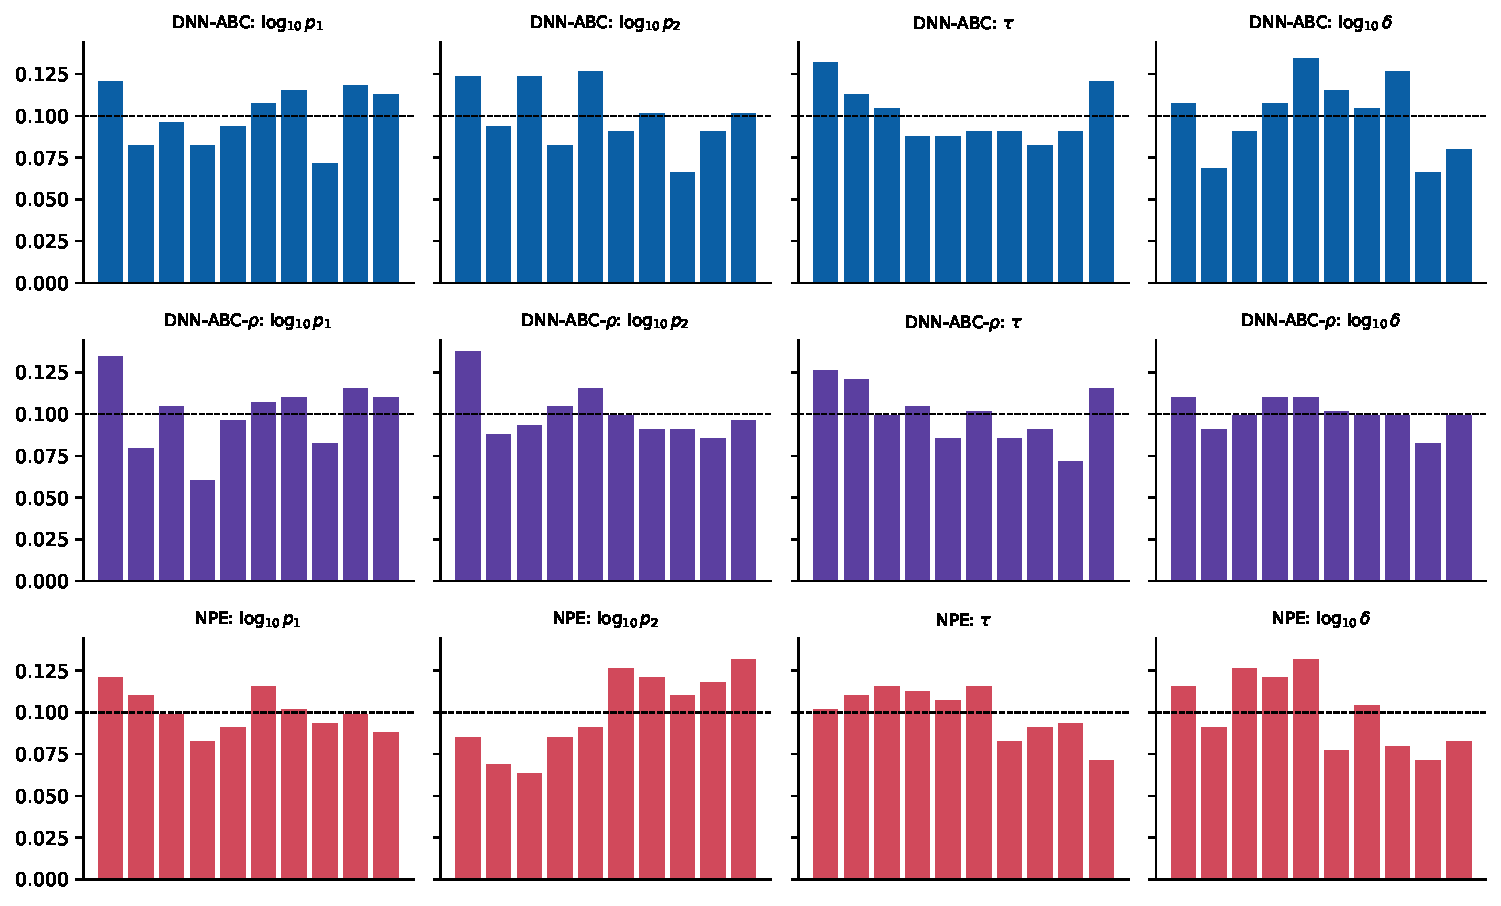
\includegraphics[width=0.95\linewidth]{4D/figures/fig_sbc_4d.pdf}
\caption{Simulation-based calibration rank histograms for DNN-ABC (top), DNN-ABC-$\rho$ (middle) and NPE (bottom), on the data sets with $\bar d>0$; dashed line is the uniform level.}
\label{sfig:sbc}
\end{figure}

\end{document}
